\chapter{Literature Review} \label{chap:litReview}

\section{The benefits of an adaptive behaviour state}

Children like robots, are more forgiving when a mistake or incoherence takes place. Moreover, they are quicker to ascribe human characteristics and personalities to robots \cite{beran2011understanding}. This is the reason behind the fact that child-robot interaction has enough potential to take place for a longer period of time. However, \cite{kanda2007two} has shown that for persistent interaction between a robot and a child, it is positive that the child establishes a social bond with the robot. 

Forming a social bond is a complicated process, and this can only be done through the expression of feelings, emotions and adaptive gestures. These expressions are very important in interactions and the forming of social relationships \cite{butler2003social}\cite{mcneill1992hand}. Hopefully, several studies, among them \cite{leite2012modelling} show that empathy facilities interaction in robot-child interaction, showing that human-based expressions can be successfully implemented by robots. Section \ref{models} goes deep in the current models for this topic.

Based on the previous statements, \cite{beran2011understanding} established that we can influence the expressive behavior of children by adapting the emotion expression of their robotic interaction partner. And the results obtained were that, children show more positive expressions with an affective robot. We can also state that children enjoy themselves more with a robot which shows adaptive behaviour expressions and gestures rather than with a robot which does not.

However, there are some constraints in the interaction to be taken into account. For instance, \cite{beran2011understanding} also established that children particularly prefer a robot which shows emotion through movement, whereas showing emotion through voice has the negative effect of reducing intelligibility.

\section{Behaviour expression models} \label{models}
In emotion research field there are two main established approaches. The first of them is based on distinguish several basic universal emotions such as happiness and sadness that implicitly assumes a discretization of the emotion. The second one considers an emotion to be a combination of two concepts: valence and arousal.
Arousal could be define as how exiting the emotion is, having several degrees of intensity whereas valence, would be how positive or negative the emotion is perceived. This approach as difference of the previous one, assumes a continuous space allowing the design of complex emotional states and smoothed transitions.
In both cases the models have some biological evidences. If we consider for instance a prolonged relaxed and quite situation without the influence of any external factor, new emotions take over the previous one within a certain period of time. However, external factors can make human switch from happiness to sadness: a bad new or a defeat for instance, as the first model suggests.
Therefore, the most important design choice is to have either a functional or a biological inspired approach. If we consider that the robot reacts directly from the environment, then it is functional but if it reacts according to its internal state, which is influenced by the environment, becomes biological inspired. Studies like \cite{schulte1999spontaneous} employs a state-machine based solution, but the recent tendency is to go towards a long-term interaction driven by the existence of an internal state \cite{hirth2011towards} \cite{canamero2001show}.
Tielman et al. for instance, proposed a model \cite{tielman2014adaptive} based on both by separation between gestures and emotion externalization consisting in four phases: an input phase, adapting the internal parameters based on this input, reasoning about the correct behaviour and the output to the robot. Recent works \cite{lim2014mei} focus more on a the feature acquisition from the environment. Features often related with the voice such as pitch volume or intensity.
However, another more complex models have been formulated. An example is \cite{velasquez1998modeling} which divides the releasers of emotion into four different complex neural mechanisms simulations: neural, sensorimotor, motivational and cognitive. In \cite{breazeal2003emotion} external events such as visual and auditory stimuli are sensed by the robot and are filtered by a number of feature extractors (e.g., color, motion, pitch, etc.). Then, in a high-level perceptual system, these features are bound by releaser processes that encode the robot's current set of beliefs about the state of the robot and its relation to the world.
\\
\section{The behaviour expression in child-robot interaction}

The use of behaviour and emotion externalization is a common resource to enhance interaction in educational, recreative and sometimes both contexts combined. The importance of this human feature is that relevant that several European projects, among them EMOTE\footnote{http://www.emote-project.eu/}, aims to improve the use of artificial tutors as learning-facilitator tools. The reason is that current platforms fail to engage the students in the same way a teacher does, as they lack the personal and empathy elements. Their research "explores how the exchange of emotional cues with an artificial tutor can create a sense of connection and act as a facilitator of the learning experience".
A commercial example of an interactive emotive robot is the owl ixi-play from WittyWorX (figure \ref{fig:int1}). It is an engaging robot buddy offering a simply playful interaction in the form of tangible games for early stage children. It is based on a peer situation where they play different games with in an active and adaptive manner. 
Pereira et al. in 2008 \cite{pereira2008icat} through an experiment consisting in to two scenarios: The first one, the user played against a physically embodied robotic agent (figure \ref{fig:int2}) and the second one, against a virtually embodied agent displayed on a screen proving that embodiment and emotion expression has implications on user enjoyment. 
The almost standard scenario of peer-to-peer set-up child-robot interaction, has evolved towards the inclusion of tactile displays that allows the execution of a rich number of activities equalizing the level of participation. An example is shown in figure \ref{fig:int3} from \cite{belpaeme2012multimodal}, an study carry out in the context of the project ALIZ-E.


\begin{figure}[h!]
        \centering
        \begin{subfigure}[b]{0.4\textwidth}
                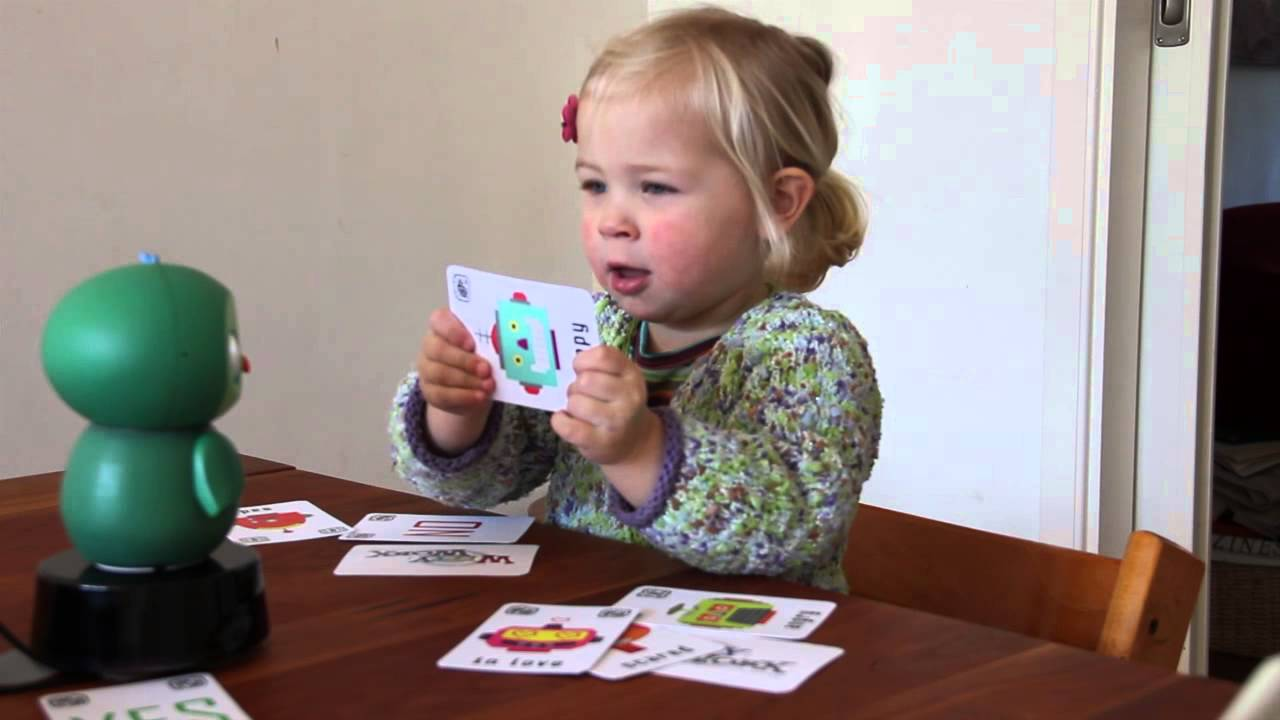
\includegraphics[width=\textwidth]{figures/int1.jpg}
                \caption{ixi-play}
                \label{fig:int1}
        \end{subfigure}%
        ~ %add desired spacing between images, e. g. ~, \quad, \qquad, \hfill etc.
          %(or a blank line to force the subfigure onto a new line)
        \begin{subfigure}[b]{0.475\textwidth}
                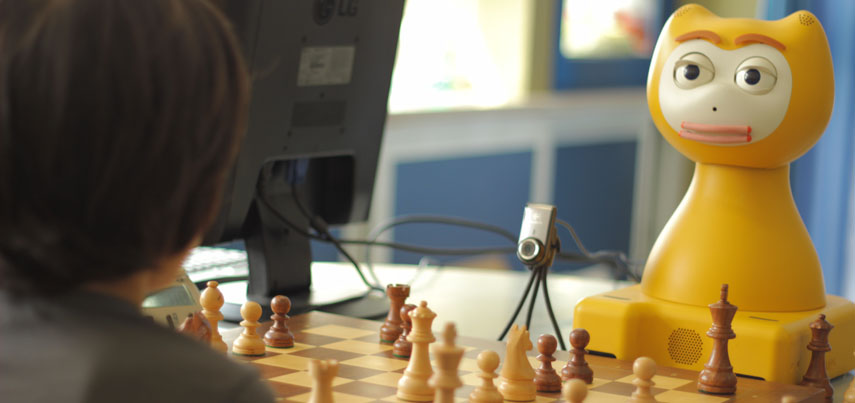
\includegraphics[width=\textwidth]{figures/int2.jpg}
                \caption{iCat}
                \label{fig:int2}
        \end{subfigure}
        ~ %add desired spacing between images, e. g. ~, \quad, \qquad, \hfill etc.
          %(or a blank line to force the subfigure onto a new line)
        \begin{subfigure}[b]{0.3\textwidth}
                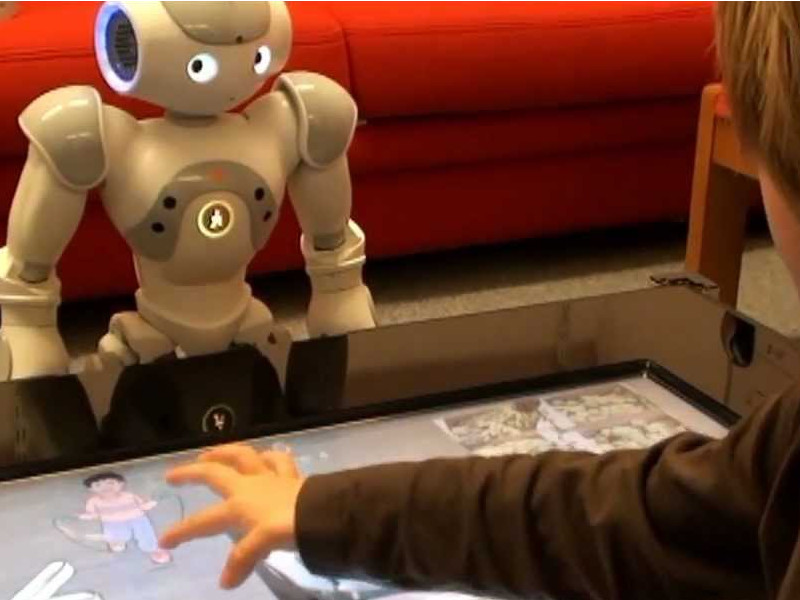
\includegraphics[width=\textwidth]{figures/int3.jpg}
                \caption{Nao}
                \label{fig:int3}
        \end{subfigure}
        \caption{Example results from emotion expression in child-robot interactions}\label{fig:animals}
\end{figure}

\section{The learning by teaching paradigm} \label{learningby}

In the learning by teaching paradigm, a student takes on the role of a teacher in order to teach
another student, and hopefully learns especially well as a result (such as in \cite{palinscar1984reciprocal}). Rohrbeck et al. \cite{rohrbeck2003peer} in their meta-analytic review of 81 peer tutoring programs in elementary schools, stated that peer-assisted learning interventions “effectively engage students in the learning process and produce academic gains across a variety of student populations, academic subjects, and classroom arrangements.”

Learning by teaching may be extended to involve a student teaching another who is not
a human, but rather a teachable agent which simulates a naive learner therefore motivating
students to teach it. Teachable agents have the benefits that they cause a student to reflect
on their knowledge and increase their ability of self-explanation; that they help the student to
structure/reorganize their knowledge; and that the student is promoted to take responsibility
of learning \cite{zhao2012learning}.

Okita and Schwartz \cite{okita2006observation} note that, given that a student has sufficient pre-understanding to interpret the actions of someone that they are observing, any discrepancies between what the student understands and what is seen in another’s actions may alert them to think more deeply about who is correct. It is reasonable to suspect that these discrepancies might not just be in the final result of the action observed: that is, when teaching another how to write, it may not just
be discrepancies in the final shape that act as a trigger for reflection in the teaching pupil, but
also the process of writing which was observed. This provides reasoning for having a teachable
agent which is sufficiently embodied so as to facilitate this.

While \cite{zhao2012learning} recommends the development of a teachable agent that is actively, rather than passively, engaged in the learning by teaching interaction, the increased learning gain results attained in \cite{okita2006observation} were done so even with the pupil being taught having been instructed to not contribute much information. This suggests that it may not be necessary, from a learning by teaching point of view, for the teachable agent to participate actively in the interaction to incite educational benefits. However, from an engagement point of view, this may not necessarily be true.

\section{The CoWriter project}
The CoWriter project\footnote{https://github.com/chili-epfl/cowriter\_letter\_learning/} involves the development of the first known robotic agent which can engage a user in the learning by teaching paradigm for handwriting. By leveraging simulated handwriting on
a synchronised tablet display, a Nao humanoid robot with limited fine motor capabilities is configured as a suitably embodied handwriting partner (see figure \ref{fig:cowriter}).

\begin{figure}[h!]
        \centering
        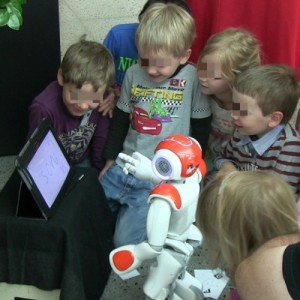
\includegraphics[width=0.4\textwidth]{figures/cowriter.jpg}
        \caption{CoWriter set-up.}
        \label{fig:cowriter}
\end{figure}

In order to achieve the simulated handwriting, shape models derived from principal component analysis of a dataset of letter trajectories are generated to parametrise written characters in a way that captures intuitively significant properties. Such a learning algorithm was developed, capable of incorporating feedback from users, both in terms of which generated letters are the best and from user demonstrations. Some of the most relevant tools used for the implementation of the system are reviewed in chapter \ref{chap:tools}.



